\documentclass[tikz,border=7pt]{standalone}
\begin{document}
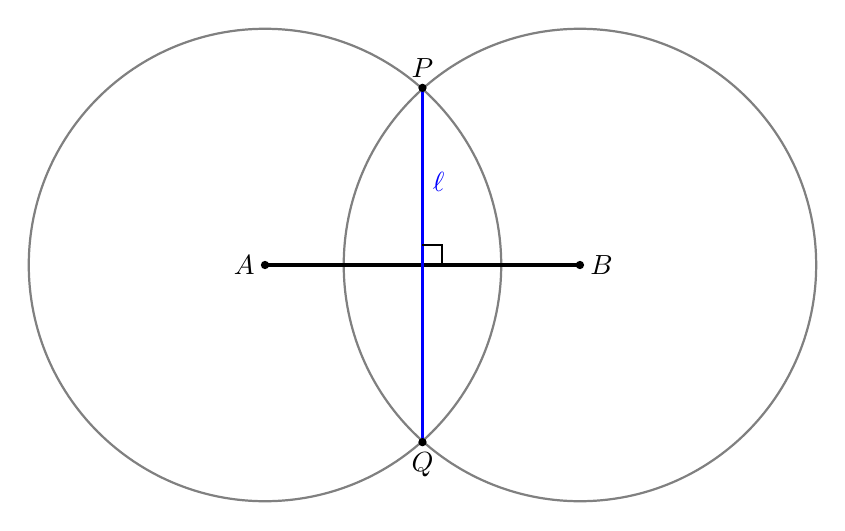
\begin{tikzpicture}[line width=.8pt]
\coordinate (A) at (-2,0); \coordinate (B) at (2,0); \coordinate (P) at (0,2.25); \coordinate (Q) at (0,-2.25);
\draw[gray] (A) circle (3); \draw[gray] (B) circle (3);
\draw[very thick] (A)--(B); \draw[blue,very thick] (P)--(Q);
\foreach \p/\pos in {A/left,B/right,P/above,Q/below} \fill (\p) circle (1.5pt) node[\pos] {$\p$};
\draw (0,.25)--(.25,.25)--(.25,0);
\node[blue,right] at (0,1.05) {$\ell$};
\end{tikzpicture}
\end{document}
